
\documentclass{beamer}
\usepackage{graphicx}
\usepackage{amsmath,amssymb,amstext,amsthm,xargs}
\usepackage{amsfonts}
\usepackage{bbm}
\usepackage{beamerthemesplit}

\usepackage[utf8]{inputenc}
\usepackage[french]{babel}
\usepackage{bbm}

\usetheme{Antibes}
\mode<presentation>
\useoutertheme{tree}
\usecolortheme{beaver}
\useinnertheme{rectangles}

\setbeamerfont{block title}{size={}}
%\usecolortheme[rgb={0.55,0.1,0.05}]{structure}
%\usecolortheme[rgb={0.75,0.1,0.05}]{structure}
\usepackage{color}

\newenvironment{disarray}{\everymath{\displaystyle\everymath{}}\array} {\endarray}
\newtheorem{theo}{Théorème}
\newtheorem{prop}[theo]{Proposition}
\newtheorem{conj}[theo]{Conjecture}
\newtheorem{cor}{Corollary}[theo]

\newtheorem{lem}{Lemme}
\newtheorem{nota}{Notation}
\newtheorem{rk}{Remark}
\newtheorem{exa}{Example}
\newtheorem{df}{Definition}
\newtheorem{terminologie}{Terminologie}
\def\rme{\mathrm{e}}
\def\rmi{\mathrm{i}}
\def\rset{\mathbb{R}}
\def\nset{\mathbb{N}}
\def\dlim{\stackrel{d}{\rightarrow}}
\newcommandx{\plim}[1][1=]{\stackrel{\PP_{#1}}{\longrightarrow}}
\def\iid{i.i.d.}
\def\1{\mathbbm{1}}
\newenvironment{dem}{\textbf{Proof}}{\flushright$\blacksquare$\\}
%\def\blankframe{
%\mode<presentation>{
%  { \setbeamertemplate{background canvas}[default]
%    \setbeamercolor{background canvas}{bg=black}
%    \begin{frame}[plain]{}
%    \end{frame}
%  }
%}
%\mode<presentation>{
%\setbeamertemplate{background canvas}[default]
%\setbeamercolor{background canvas}{bg=white}}
%\mode*
%}
\def\eqsp{\,}
\DeclareMathOperator{\E}{{\mathbb E}}
\def\PE{\E}
\def\PCov{\mathrm{Cov}}
\DeclareMathOperator{\F}{{\mathbb F}}
\DeclareMathOperator{\G}{{\mathbb G}}
\DeclareMathOperator{\D}{{\mathbb D}}
\DeclareMathOperator{\R}{{\mathbb R}}
\DeclareMathOperator{\C}{{\mathbb C}}
\DeclareMathOperator{\Z}{{\mathbb Z}}
\DeclareMathOperator{\N}{{\mathbb N}}
\DeclareMathOperator{\K}{{\mathbb K}}
\DeclareMathOperator{\T}{{\mathbb T}}
\DeclareMathOperator{\PP}{{\mathbb P}}
\DeclareMathOperator{\QQ}{{\mathbb Q}}
\DeclareMathOperator{\Q}{{\mathbb Q}}
\DeclareMathOperator{\IF}{{\mathbb I}}


%%%%%%%%%%%%%%%%%%%%%%%%%%%%%%% Pour le modèle lin\'eaire

\DeclareMathOperator{\bX}{\boldsymbol{X}}
\DeclareMathOperator{\bY}{\boldsymbol{Y}}
\DeclareMathOperator{\bx}{\boldsymbol{x}}
\DeclareMathOperator{\vp}{\boldsymbol{p}}
\DeclareMathOperator{\vq}{\boldsymbol{q}}
\DeclareMathOperator{\estMCNL}{\widehat \theta_n^{\,\,{\tt mcnl}}}
\DeclareMathOperator{\estMV}{\widehat \theta_n^{\,\,{\tt mv}}}
\DeclareMathOperator{\est}{\widehat \theta_{\mathnormal{n}}}
\DeclareMathOperator{\var}{\mathrm{Var}}
\def\Var{\var}
\DeclareMathOperator{\estMVc}{\widehat \theta_{n,0}^{\,{\tt mv}}}
\DeclareMathOperator{\Xbar}{\overline{\mathnormal{X}}_\mathnormal{n}}

\newcommand{\indi}[1]{\mathbbm{1}_{\{#1\}}}
\newcommand{\coint}[1]{\left[#1\right)}
\newcommand{\ocint}[1]{\left(#1\right]}
\newcommand{\ooint}[1]{\left(#1\right)}
\newcommand{\ccint}[1]{\left[#1\right]}

\definecolor{LightYell}{rgb}{0.95,0.83,0.70}
\definecolor{orange}{rgb}{1.0,0.50,0.01}
\definecolor{StroYell}{rgb}{0.95,0.88,0.72}
\definecolor{lightred}{rgb}{0.75,0.033,0}
\definecolor{shadecolor1}{rgb}{0.90,0.83,0.70}
\definecolor{myem}{rgb}{0.797,0.598,0.598}
\definecolor{BrickRed}{cmyk}{0,0.89,0.94,0.28}
\definecolor{RoyalPurple}{cmyk}{0.75,0.9,0,0}

\newcommand{\tco}[1]{\textcolor{orange}{#1}}
\newcommand{\tcr}[1]{\textcolor{lightred}{#1}}

\def\gauss{\mathcal{N}}
\def\truetheta{\theta}
\def\truebeta{\boldsymbol{\beta}}
\def\projX{A}
\def\curtheta{\alpha}
\def\argmin{\mathrm{argmin}}
\def\ie{\emph{i.e.}}
\def\regressmat{\mathbb{X}}
\def\errpred{\boldsymbol{\hat{\xi}}}
\def\bnoise{\boldsymbol{\xi}}
\def\predY{\hat{\mathbf{Y}}}
\DeclareMathOperator{\estregress}{\widehat{\truebeta}_n}
\DeclareMathOperator{\estMC}{\widehat \theta_n^{\,\,{\tt mc}}}
\def\curbeta{b}
\def\bcurbeta{\mathbf{b}}
\newcommand{\indep}{\rotatebox[origin=c]{90}{$\models$}} 
\newcommand{\Id}[1]{\mathrm{Id}_{#1}}

\title{MAP 433 : Introduction aux méthodes statistiques. Cours 8}
%\author{M. Hoffmann}
%\institute{Université Paris-Est and ETG}
\begin{document}
\date{16 Octobre 2015}
\maketitle



\begin{frame}
\frametitle{Aujourd'hui}
\tableofcontents
\end{frame}

\section{Le modèle de régression: quelques rappels}
\begin{frame}
\frametitle{Modèle de régression}
\begin{df}
Données: $(\bx_1,Y_1),\ldots, (\bx_n,Y_n)$ avec $Y_i \in \R, \bx_i\in \R^k$, et
$$Y_i =
r(\alert{\truebeta},\bx_i)+ \sigma \xi_i,\;\;\E_{\truetheta}\big[\xi_i\big]=0,
$$
\begin{itemize}
%\item $\bx \leadsto r(\alert{\truetheta},\bx)$ fonction de \alert{ régression}, connue au paramètre
%$\truetheta$ près.
\item \alert<1>{$\bx_i$ déterministes, donnés (ou choisis) : plan d'expérience.}
\item \alert<2>{Hypothèses sur les $\xi_i$ : à débattre. \alert{Pour simplifier}, les variables $\xi_i$ sont centrées, $\PE_{\truetheta}[\xi_i]=0$,
décorrélées, $\PE_{\truetheta}[\xi_i \xi_j]= 0$ si $i \ne j$ et de variance unité $\PE[\xi_i^2]= 1$ \alert{ (homoscédasticité)}.}
\item \alert<3>{ Attention ! Les $Y_i$ ne sont pas identiquement distribuées.}
\item \alert<4>{$\truetheta= (\truebeta,\sigma^2) \in  \R^d \times \R_+.$}
\end{itemize}
\end{df}


\end{frame}

\begin{frame}
\frametitle{Régression gaussienne}


\begin{itemize}
\item  Modèle de régression:
$$Y_i =
r({\truebeta},\bx_i)+\ \sigma \xi_i,\;\;\truetheta \in \Theta\subset  \R^d \times \rset_+.$$
\item  Supposons: $\xi_i \sim {\mathcal N}(0,1)$, i.i.d.
\item On a alors le modèle de \alert{régression gaussienne}.
Comment estimer $\truetheta$?  \alert{On sait expliciter la loi
de l'observation} $Z=(Y_1,\dots,Y_n)$ $\Longrightarrow$ appliquer le
principe du maximum de vraisemblance.

\item La loi de $Y_i$:
\begin{align*}
\PP^{Y_i}(dy) & = \frac{1}{\sqrt{2\pi \sigma^2}}\exp\big
(-\frac{1}{2\sigma^2}(y-r({\truebeta},\bx_i))^2\big)dy \\
& \ll dy.
\end{align*}

%d'où
%$$\PP^{(Y_1,\ldots, Y_n)}(dy_1\ldots dy_n) = \Big(\prod_{i=1}^n \frac{1}{\sqrt{2\pi \sigma^2}}\exp\big(-\frac{1}{2\sigma^2}(y-\truetheta^T\bx_i)\big)\Big) dy_1\ldots dy_n$$
\end{itemize}
\end{frame}

\begin{frame}
\frametitle{EMV pour régression gaussienne}
\begin{itemize}
\item  Le modèle $\{\PP_\truetheta^n \alert{ = \text{loi de }\;(Y_1,\ldots, Y_n)},\truetheta = (\truebeta,\sigma^2) \in \R^k \times \rset_+^* \}$ est \alert{dominé} par
$\mu^n(dy_1\ldots dy_n) = dy_1\ldots dy_n.$
\item D'où
\[
 \frac{d\PP_\truetheta^n}{d\mu^n}(y_1,\ldots, y_n)
  =\; \prod_{i=1}^n \tfrac{1}{\sqrt{2\pi \sigma^2}}\exp
  \big(-\tfrac{1}{2\sigma^2}(y_i-r({\truebeta},\bx_i))^2\big)
%\;= & \tfrac{1}{(\sqrt{2\pi \sigma^2})^{n}}
%\exp\big(-\tfrac{1}{2\sigma^2}\sum_{i =
%1}^n\big(y_i-r({\truebeta},\bx_i)\big)^2\big).
\]
\item La fonction de vraisemblance
$$\boxed{{\mathcal L}_n(\truetheta, Y_1,\ldots, Y_n)
= \tfrac{1}{(\sqrt{2\pi \sigma^2})^{n}} \exp\Big(-\frac{1}{2\sigma^2}\sum_{i = 1}^n\big(Y_i-
r({\truebeta},\bx_i)\big)^2\Big)}$$
\end{itemize}
\end{frame}

\begin{frame}
\frametitle{Estimateur des moindres carrés}
Maximiser la
\alert{ vraisemblance} en régression gaussienne
\begin{align*}
\estregress &\in \argmin_{\curbeta \in \rset^k} \sum_{i = 1}^n \big(Y_i-r(\curbeta,\bx_i)\big)^2 \\
\hat{\sigma}_n^2 &= n^{-1} \sum_{i=1}^n (Y_i - r(\estregress,\bx_i))^2
\end{align*}
%\begin{df}
%Estimateur des \alert{moindres carrés} : tout estimateur
%$\estregress$ t.q. \centerline{$\estregress \in \arg \min_{\truebeta \in
%\Theta}\sum_{i = 1}^n \big(Y_i-r({\truebeta},\bx_i)\big)^2.$}
%\end{df}
\begin{itemize}
\item  L'estimateur $\estregress$ est appelé l'\alert{estimateur des moindres carrés}. Il peut être appliqué même dans un cas non gaussien.
\item \alert{ Existence, unicité.}
\end{itemize}
\end{frame}


\subsection{Régression linéaire multiple}

\begin{frame}
\frametitle{Régression linéaire multiple (=Modèle linéaire)}
\begin{itemize}
\item La fonction de régression est $r(\truebeta,\bx_i) = \bx_i^T \truebeta$.
On observe
$$(\bx_1,Y_1),\ldots, (\bx_n,Y_n)$$
avec
$$\boxed{Y_i = \bx_i^T \truebeta+ \sigma \xi_i,\;\;i=1,\ldots, n}$$
où $\truetheta \in \Theta = \R^k,\;\;\bx_i \in \R^k$.
\item \alert{Matriciellement}
$$\boxed{\bY = \regressmat\truebeta + \sigma \bnoise}$$
avec
\begin{itemize}
\item \alert<1>{$\bY = (Y_1 \cdots Y_n)^T$},
\item \alert<2>{$\bnoise = (\xi_1 \cdots \xi_n)^T$}
\item \alert<3>{$\regressmat$ la matrice $(n\times k)$
dont la $i$-ème ligne est $\regressmat_{i,\cdot}= \bx_i^T$.}
\end{itemize}
\end{itemize}
\end{frame}

\begin{frame}
\frametitle{EMC en régression linéaire multiple}
\begin{itemize}
\item Estimateur des \alert{moindres carrés} en régression
linéaire multiple : tout estimateur $\estregress$ satisfaisant
$$\sum_{i = 1}^n
\big(Y_i- \bx_i^T \estregress \big)^2 = \min_{\bcurbeta \in \R^k}\sum_{i =
1}^n \big(Y_i- \bx_i^T \bcurbeta\big)^2.$$
\item En notation matricielle :
\begin{align*}
\|\boldsymbol{Y}-\regressmat\estregress\|^2 &=   \min_{\bcurbeta \in \R^k}\|\bY -\regressmat\truebeta\|^2\\
&= \min_{v \in V}\|\boldsymbol{Y}-v\|^2
\end{align*}
o\`u $V=\text{Im}(\regressmat) = \{v\in \R^n: v=\regressmat \bcurbeta, \
\bcurbeta \in \R^k\}$. \alert{Projection orthogonale sur $V$}.
\end{itemize}
\end{frame}

% \subsection{Géometrie de l'EMC}

 \begin{frame}
\frametitle{Géométrie de l'EMC}
 \begin{itemize}
 \item L'EMC vérifie
$$\boxed{\regressmat \estregress = P_V \boldsymbol{Y}}$$
o\`u $P_V$ est le projecteur orthogonal sur $V$.
\item Comme $ \bY - P_V \bY \perp V$, on en déduit \alert{les équations normales des
moindres carrés}:
$$\boxed{\regressmat^T\regressmat {\estregress} =
\regressmat^T\boldsymbol{Y}.}$$
\item \underline{Remarques.}
  \begin{itemize}
  \item L'EMC est un $Z$-estimateur.
  \item \alert{unicité} de $\estregress$ si la matrice de Gram
  $\regressmat^T\regressmat$ est inversible (la matrice $\regressmat$ est de rang complet).
  \end{itemize}
\end{itemize}
\end{frame}

\begin{frame} \frametitle{Géométrie de l'EMC}
\begin{prop}
Si $\regressmat^T\regressmat$ (matrice $k \times k$) inversible, alors
$\estregress$ \alert{est unique} et
$$\boxed{\estregress = \big(\regressmat^T\regressmat\big)^{-1}\regressmat^T \boldsymbol{Y}}= \regressmat^{\#} \bY$$
\end{prop}
$$
\projX = \regressmat\big(\regressmat^T\regressmat\big)^{-1}\regressmat^T = \regressmat \regressmat^{\#}
$$
est dite \alert{matrice chapeau} (\texttt{hat matrix}).
%
\begin{prop}
Si $\regressmat^T\regressmat>0$, alors $\projX$ est le projecteur sur
$V$: \alert{$\projX=P_V$} et \alert{${\rm rang}(\projX)=k$}.
\end{prop}
\end{frame}


\subsection{Propriétés de l'estimateur des Moindres Carrés: modèle Gaussien}

\begin{frame}
\frametitle{Hypothèses}
\[
\bY= \regressmat \truebeta + \sigma \bnoise
\]
\begin{enumerate}
\item \alert<1>{$\regressmat$ est de rang complet.}
\item \alert<2>{$\bnoise \sim \gauss(0,\Id{n})$}
\end{enumerate}
\end{frame}


\begin{frame}
\frametitle{Propriétés de l'estimateur}
\begin{theo}
Pour tout $(\truebeta,\sigma^2) \in \rset^d \times \rset_+$, sous $\PP_{\truebeta,\sigma^2}$, l'estimateur
$\estregress$ est un vecteur Gaussien de moyenne $\truebeta$ et de variance $\sigma^2(\regressmat^T \regressmat)^{-1}$
\end{theo}
\begin{proof}
\begin{align*}
\estregress
&= \regressmat^{\#} \bY = \regressmat^{\#} (\regressmat \truebeta + \sigma \bnoise) \\
&= \truebeta + \sigma \regressmat^{\#} \bnoise
\end{align*}
Le vecteur $\regressmat^{\#} \bnoise$ est Gaussien centré de matrice de covariance
\[
\regressmat^{\#} \left( \regressmat^{\#} \right)^T = (\regressmat^T \regressmat)^{-1} \eqsp.
\]
\end{proof}
\end{frame}


\begin{frame}
\frametitle{Prédiction et Erreur de prédiction}
\begin{itemize}
\item \alert{Prédiction}
\[
\predY= \regressmat \estregress = \projX \bY
\]
projection des observations sur l'espace de régression.
\item \alert{Erreur de prédiction}:
\[
\errpred = \bY - \predY = (\Id{n} - \projX) \bY \eqsp.
\]
\item Sous $\PP_\truetheta$, $\bY= \regressmat \truebeta +  \sigma \bnoise$. Donc,
\begin{align*}
\predY    &= \regressmat \truebeta + \sigma \projX \bnoise \\
\errpred  &= \sigma (\Id{n}-\projX) \bnoise
\end{align*}
car $\projX \regressmat= \regressmat$ ($\projX$ est le projecteur orthogonal sur l'image de $\regressmat$).
\end{itemize}
\end{frame}


\begin{frame}
\frametitle{Théorème de Cochran}
\begin{theo}
Soit $\bY \sim N(\mu,\sigma^2 \Id{n})$, $\mathcal{M}$ un sous espace de $\R^n$ de dimension $k$, $\Pi$ la matrice de projection orthogonale
sur $\mathcal{M}$ et $\Pi_{\perp}= \Id{n} - \Pi$ la matrice de projection orthogonale sur $\mathcal{M}^\perp$. Nous avons
\begin{enumerate}
\item \alert<1>{$\Pi \bY \sim \gauss(\Pi \mu, \sigma^2 \Pi)$, $\Pi_\perp \bY \sim \gauss(\Pi_{\perp} \mu, \sigma^2 \Pi_{\perp})$}
\item \alert<2>{les vecteurs $\Pi \bY$ et $\Pi_\perp \bY$ sont indépendants}
\item \alert<3>{$\| \Pi(\bY - \mu) \|^2 / \sigma^2 \sim \chi^2_k$ et $\Pi_\perp(\bY-\mu) \|^2/\sigma^2 \sim \chi^2_{n-k}$}.
\end{enumerate}
\end{theo}
\end{frame}

\begin{frame}
\frametitle{Résidus et variance résiduelle}
Sous $\PP_{\truebeta,\sigma^2}$, $\bY= \regressmat \truebeta +  \sigma \bnoise$,
\begin{align*}
\estregress    &=  \truebeta + \sigma \regressmat^{\#} \bnoise \\
\errpred       &= \sigma (\Id{n}-\projX) \bnoise \\
\hat{\sigma}^2 &= (n-k)^{-1} \| \errpred \|^2
\end{align*}
\begin{theorem}
Pour tout $(\truebeta,\sigma^2) \in \rset^k \times \rset_+$,
\begin{enumerate}
\item $(n-p) \hat{\sigma}^2/\sigma^2$ suit une loi du $\chi^2$ à $(n-k)$ degrés de liberté.
\item $\estregress$ et $\hat{\sigma}^2$ sont indépendants.
\end{enumerate}
\end{theorem}
\begin{proof}
\only<1>{
$(\Id{n}- \projX) \bnoise \sim \gauss(0,(\Id{n}-\projX))$ et donc $\|(\Id{n}- \projX) \bnoise\|^2$ suit une loi du $\chi^2$ à
$(n-k)= \mathrm{Tr}(\Id{n} - \projX)$ d.l.
}
\only<2>{
$$
\estregress= \truebeta +  \sigma \regressmat^{\#} \bnoise = \truebeta + \sigma \regressmat^{\#} \projX \bnoise
$$
et $ \projX \bnoise$ et $(\Id{n}- \projX) \bnoise$ sont indépendants.
}
\end{proof}
\end{frame}

\begin{frame}
\frametitle{Loi de Student}
\begin{definition}
Soit $Z$ une variable aléatoire de loi normale centrée et réduite et soit $U$ une variable indépendante de $Z$ et distribuée suivant la loi du
$\chi^2$ à $p$ degrés de liberté.
Par définition la variable
\[
T = \frac{Z}{\sqrt{U/p}}
\]
suit une loi de Student à $p$ degrés de liberté.
\end{definition}
\end{frame}

\begin{frame}
\frametitle{Loi de Fisher}
\begin{definition}
 Soient $U_1$ et  $U_2$ deux variables aléatoires indépendantes distribuées  selon une Loi du $\chi^2$ à $d_1$ et $d_2$ degrés de liberté.
Par définition, la variable
\[
 \frac{U_1/d_1}{U_2/d_2}
\]
est distribuée suivant une loi de Fisher à $(d_1,d_2)$ d.l.
\end{definition}
\end{frame}

\begin{frame}
\frametitle{Lois des estimateurs}
\begin{theo}
Pour tout $(\truebeta,\sigma^2) \in \rset^k \times \rset_+$,
\begin{enumerate}
\item Pour $j=1,\dots,k$,
\[
T_j= \frac{\hat{\beta}_j- \beta_j}{\hat{\sigma}\sqrt{[(\regressmat^T \regressmat)^{-1}]_{j,j}}} \sigma \mathcal{T}_{n-p}
\]
\item Soit $R$ une matrice ($q \times k$) de rang $q$ ($q \leq k$) alors
\[
\frac{1}{q \hat{\sigma}^2} (R\{\estregress-\truebeta\})^T \left[ R (\regressmat^T \regressmat)^{-1} R^T \right]^{-1} R\{\estregress-\truebeta\}
\sim \mathcal{F}_{q,n-p}
\]
\end{enumerate}
\end{theo}
\begin{proof}
\only<1>{
\begin{itemize}
\item $\hat{\beta}_j- \beta_j \sim \gauss(0, \sigma^2[(\regressmat^T \regressmat)^{-1}]_{j,j})$
\item $(n-k) \hat{\sigma}^2/\sigma^2$ $\chi^2(n-k)$ d.l.
\item $\hat{\beta}_j- \beta_j$ et $(n-k) \hat{\sigma}^2$ sont indépendants.
\end{itemize}
}
\only<2>{
\begin{itemize}
\item $R\{\estregress-\truebeta\} \sim \gauss( 0, \sigma^2  R (\regressmat^T \regressmat)^{-1} R^T)$
\item $(n-k) \hat{\sigma}^2$ suit une loi du $\chi^2$ à $(n-k)$-d.l.
\item $\estregress-\truebeta$ et $\hat{\sigma}^2$ sont indépendants.
\end{itemize}
}
\end{proof}
\end{frame}

\begin{frame}
\frametitle{Intervalles de confiance}
\begin{theo}
\begin{enumerate}
\item Un intervalle de confiance bilatéral de niveau $1-\alpha$,  pour un $\beta_{j}$, $j=1,\dots, p$, est donné  par
    $$
    [\hat{\beta}_{j}-t_{n-p}(1-\alpha/2)\hat{\sigma}\sqrt{[(X'X)^{-1}]_{jj}},\ \hat{\beta}_{j}+t_{n-p}(1-\alpha/2)\hat{\sigma}\sqrt{[(X'X)^{-1}]_{jj}}]
    $$
\item Un intervalle de confiance bilatéral de niveau $ 1-\alpha$, pour $\sigma^{2}$  est donné par
$$
[\frac{(n-p)\hat{\sigma}^{2}}{c_{2}},\ \frac{(n-p)\hat{\sigma}^{2}}{c_{1}}]\ \quad \text{où} \quad  \PP(c_{1}\leq\chi_{n-p}^{2}\leq c_{2})=1-\alpha.
$$
\end{enumerate}
\end{theo}
\end{frame}


\begin{frame}
\frametitle{Régions de confiance}
\begin{theo}
 Une région de confiance  pour $q$ ($q\leq k$)  param\`{e}tres $\beta_{j}$ notés $(\beta_{j_{1}},\ \cdots,\ \beta_{j_{q}})$ de niveau
 $ 1-\alpha$ est donn\'{e}e  par
$$
\left\{R\beta \in \rset^q, \frac{1}{q\hat{\sigma}^{2}}[R(\hat{\beta}-\beta)]'[R(X'X)^{-1}R']^{-1}[R(\hat{\beta}-\beta)]\leq f_{q,n-p}(1-\alpha)\right\},
$$
o\`{u} $R$ est la matrice de taille $q\times p$ dont tous les éléments sont nuls sauf les $[R]_{ij_{i}}$, $i=1,\dots,q$ qui valent 1 et $f_{q,n-p}(1-\alpha)$ est le quantile de niveau $(1-\alpha)$ d'une loi de Fisher admettant $(q,\ n-p)$ d.l.
\end{theo}
\end{frame}

\begin{frame}
\frametitle{Un exemple}
\begin{figure}
  \centering
  % Requires \usepackage{graphicx}
  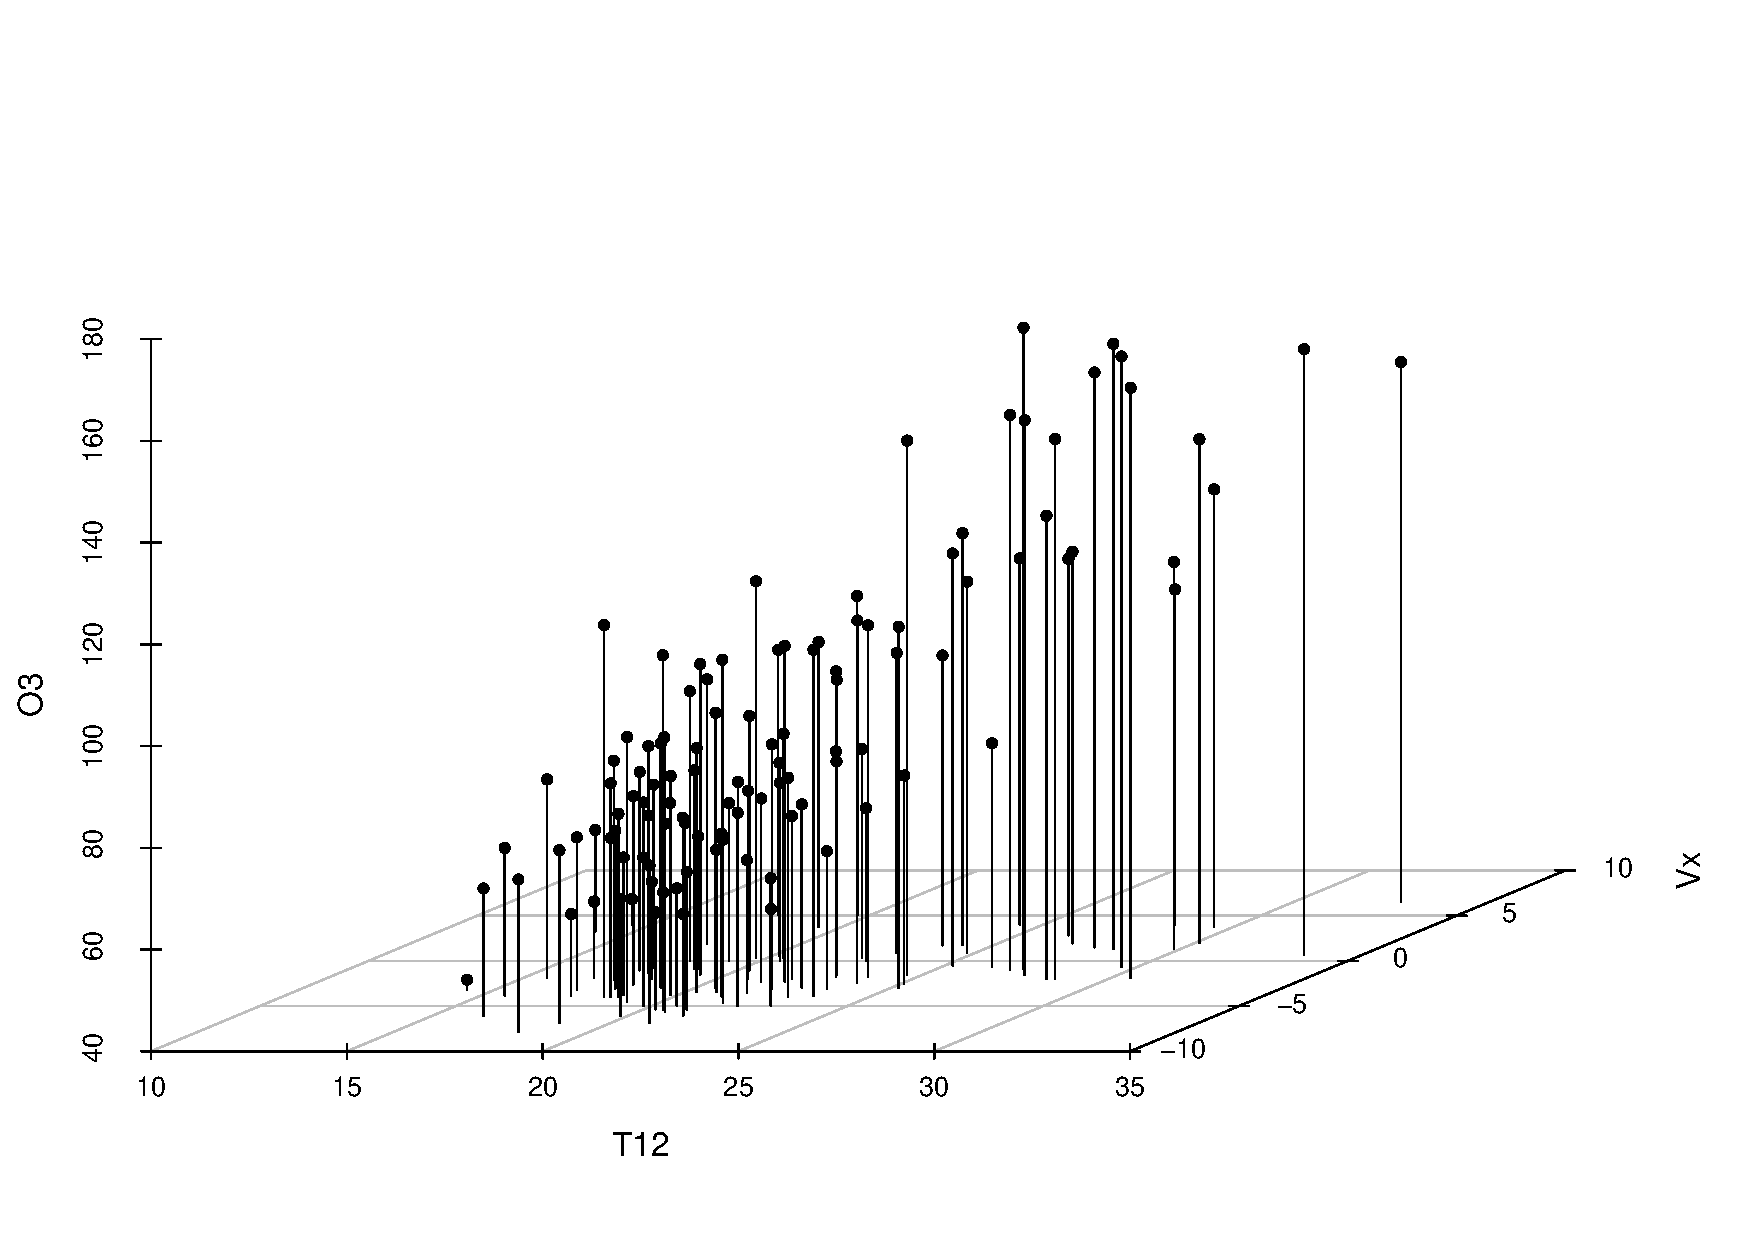
\includegraphics[width=0.8\textwidth]{ScatterPlot}\\
  \caption{Représentation brute des données: modèle d'explication de l'ozone (O3) par la température à 12h (T12) et le Vent à 12h (Vx12)}
\end{figure}
\end{frame}

\begin{frame}
\frametitle{Régression multiple}
\alert{Modèle de régression}
\[
\mathrm{maxO3}= \beta_1 + \beta_2 \mathrm{T12} + \beta_3 \mathrm{Vx12} + \beta_4 \mathrm{Ne12} + \sigma \bnoise
\]
\alert{Intervalles de confiance}
\begin{table}
\begin{tabular}{ccc}
            &      2.5 \% &   97.5 \% \\
(Intercept) &-25.4886483  & 33.280203 \\
T12         &  3.4819098  & 5.544563  \\
Vx12        &  0.3264694  & 2.931560  \\
Ne12        & -3.6368523  & 0.399082
\end{tabular}
\end{table}
\end{frame}

\begin{frame}
\frametitle{Régions de confiance}
\begin{figure}
  \centering
  % Requires \usepackage{graphicx}
  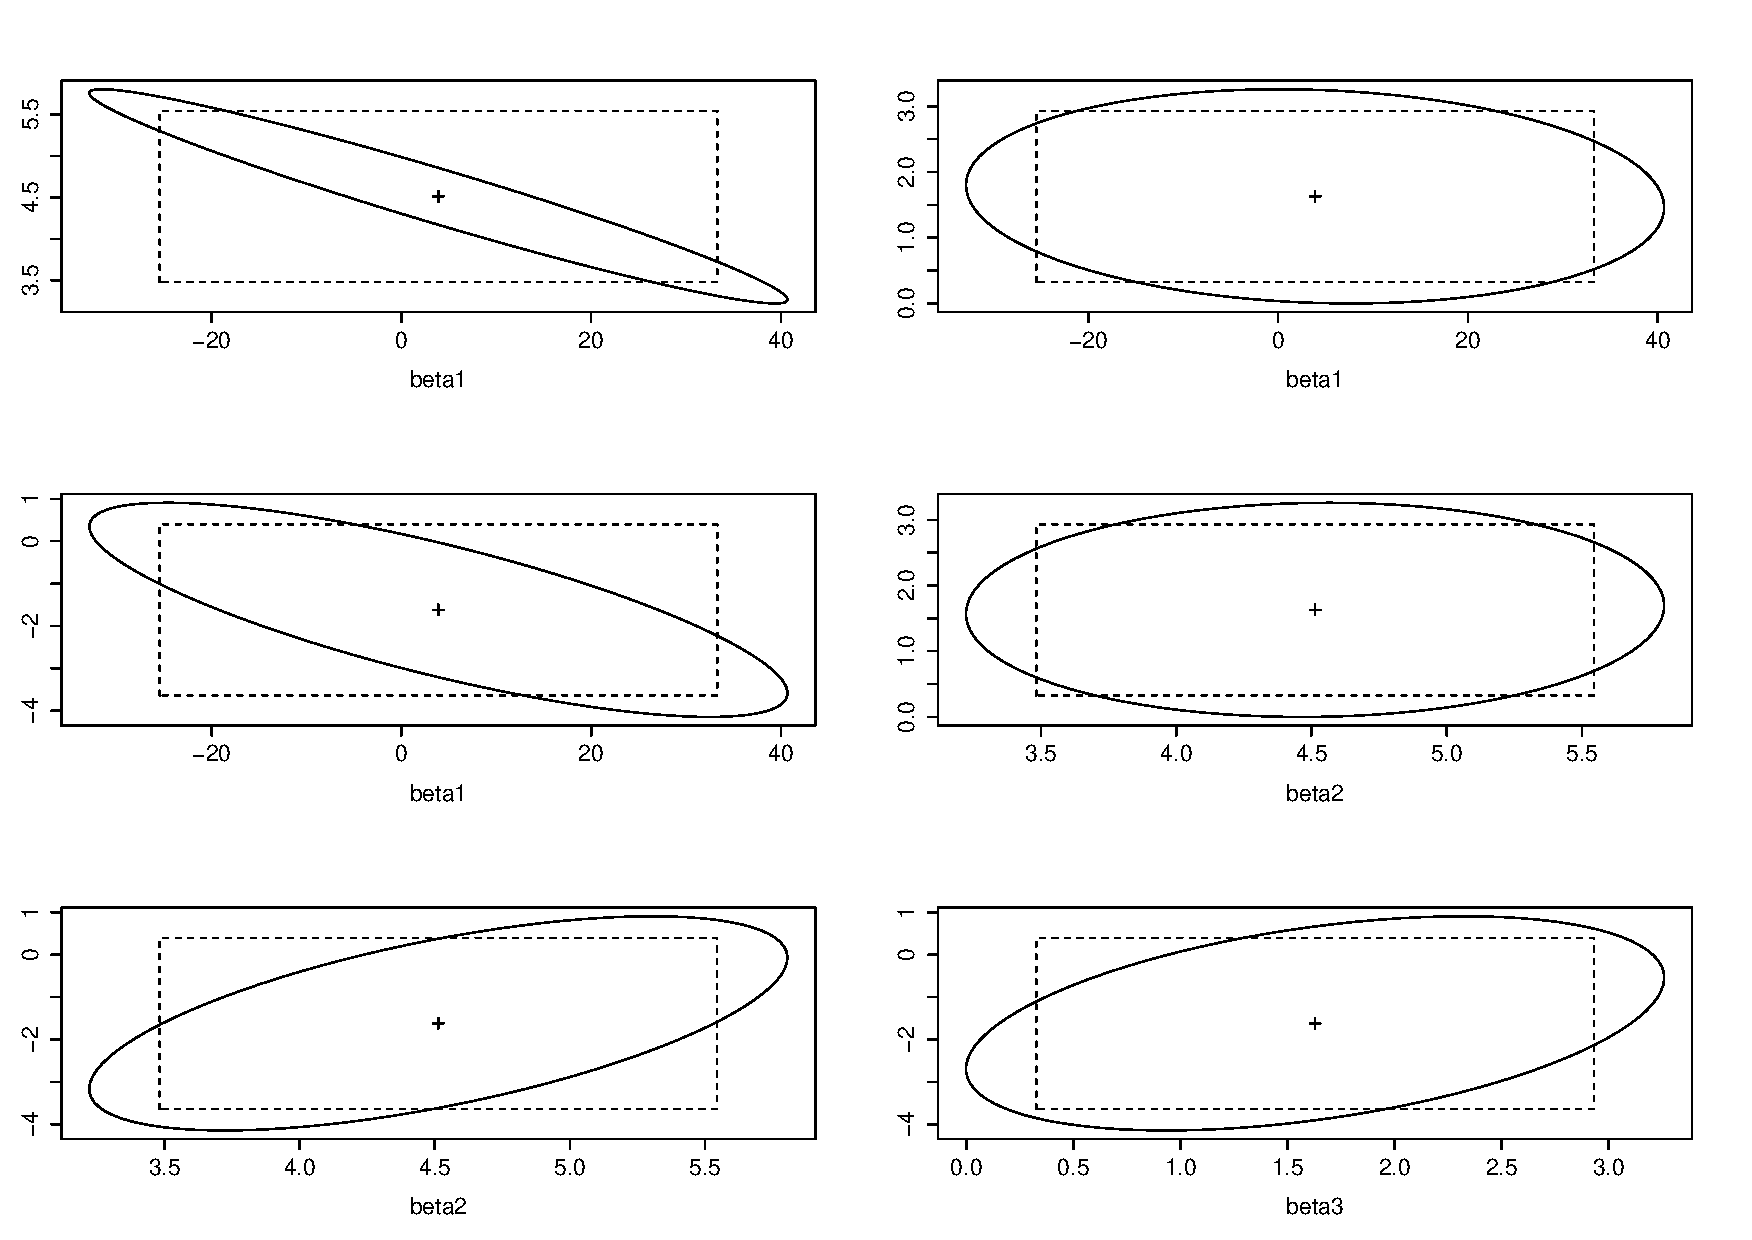
\includegraphics[width=0.8\textwidth]{Rconfiance}\\
  \caption{Régions de confiance et rectangle des couples de paramètres}
\end{figure}
\end{frame}

\section{Tests d'hypothèses}

\begin{frame}
\frametitle{Problème}
Nous avons modélisé les pics d'ozone par $\mathrm{T12}$, $\mathrm{Vx12}$ et $\mathrm{Ne12}$.
Il para\^{i}t raisonnable de se poser les questions suivantes :
\begin{enumerate}
\item Est-ce que la valeur de $\mathrm{O3}$ est influenc\'{e}e par $\mathrm{Vx}$?
\item Y a-t-il un effet n\'{e}bulosit\'{e}?
\item Est-ce que la valeur de $\mathrm{O3}$ est influenc\'{e}e par $\mathrm{Vx}$ ou $\mathrm{T12}$ ?
\end{enumerate}
Rappelons que le mod\`{e}le utilis\'{e} est le suivant:
\[
\mathrm{O3}= \beta_1 + \beta_2 \mathrm{T12} + \beta_3 \mathrm{Vx12} + \beta_4 \mathrm{Ne12} + \sigma \bnoise
\]
Nous pouvons expliciter les trois questions pr\'{e}c\'{e}dentes en terme de test d'hypo- th\`{e}se :
\begin{enumerate}
\item correspond \`{a} $\mathrm{H}_{0}:\beta_{3}=0$, contre $\mathrm{H}_{1}$ : $\beta_{3}\neq 0$;
\item  correspond \`{a} $\mathrm{H}_{0}$ : $\beta_{4}=0$, contre $\mathrm{H}_{1}$ : $\beta_{4}\neq 0$;
\item correspond \`{a} $\mathrm{H}_{0}$ : $\beta_{2}=\beta_{3}=0$, contre $\mathrm{H}_{1}$ : $\beta_{2}\neq 0$ ou $\beta_{3}\neq 0$.
\end{enumerate}
\end{frame}

\begin{frame}
\frametitle{Test entre mod\`{e}les embo\^{i}t\'{e}s}
\begin{itemize}
\item \alert{Modèle}:
$$
\text{
$\bY=\regressmat\truebeta+ \sigma \bnoise$ o\`{u} $\bnoise \sim \gauss(0,\ \sigma^{2}\Id{n})$ \eqsp,
}
$$
ce qui implique
$$ \PE_{\truebeta,\sigma^2}[\bY]= \regressmat \truebeta \in \vect(\regressmat) \eqsp.
$$
\item On cherche à tester si 
$$\PE_{\truebeta,\sigma^2}[\bY] \in \vect(\regressmat_0)
$$ 
où $\vect(\regressmat_0) \subset \vect(\regressmat)$ est un sous espace linéaire (strict) de $\vect(\regressmat)$
\item \alert{Exemple typique:} $\mathrm{H}_0$: $\beta_{j_1} = \dots = \beta_{j_q}= 0$. Dans ce cas, $\regressmat_0$ sont les colonnes
de la matrice $\regressmat$ qui correspondent aux indices $\{1,\dots,k\} \setminus \{j_1,\dots,j_q\}$
\end{itemize}
\end{frame}


\begin{frame}
\frametitle{Test du rapport de vraisemblance généralisé}
\[
\Lambda_n = \frac{\sup_{(\truebeta_0,\sigma^2)} (2 \pi \sigma^2)^{-n/2} \exp(-1/(2\sigma^2) \| \bY - \regressmat_0 \truebeta_0\|^2)}{\sup_{(\truebeta,\sigma^2)} (2 \pi \sigma^2)^{-n/2} \exp(-1/(2\sigma^2) \| \bY - \regressmat \truebeta\|^2)}
\]
\only<2>
{
\begin{itemize}
\item On calcule d'abord l'EMV sous le modèle contraint
\[
\bY = \regressmat_0 \truebeta_0 + \sigma \bnoise \eqsp.
\]
\item \alert{régresseur} $\estregress_0= \regressmat_0^{\#} \bY$, \alert{variance} $\hat{\sigma}^2= n^{-1} \| \bY - \regressmat_0 \estregress_0\|^2$
\item \alert{vraisemblance}
\[
\sup_{(\truebeta_0,\sigma^2)} (2 \pi \sigma^2)^{-n/2} \exp(-1/(2\sigma^2) \| \bY - \regressmat_0 \truebeta_0\|^2)
= \frac{exp(-n)}{(2 \pi n^{-1} \| \bY - \regressmat_0 \estregress_0\|^2)^{n/2}}
\]
\end{itemize}
}
\only<3>
{
\begin{itemize}
\item On calcule ensuite l'EMV sous le modèle non contrait
\item \alert{régresseur} $\estregress= \regressmat^{\#} \bY$, \alert{variance} $\hat{\sigma}^2= n^{-1} \| \bY - \regressmat \estregress\|^2$
\item \alert{vraisemblance}
\[
\sup_{(\truebeta,\sigma^2)} (2 \pi \sigma^2)^{-n/2} \exp(-1/(2\sigma^2) \| \bY - \regressmat \truebeta\|^2)
= \frac{exp(-n)}{(2 \pi n^{-1} \| \bY - \regressmat \estregress \|^2)^{n/2}}
\]
\end{itemize}
}
\only<4>
{
\begin{itemize}
\item En posant $\predY= \regressmat \estregress$ et $\predY_0= \regressmat_0 \estregress_0$, le RVG est donné par
\begin{align*}
\Lambda_n &= \frac{\| \bY - \predY \|^n}{\| \bY - \predY_0 \|^n}
\end{align*}
\item $\predY - \predY_0 \in \vect(\regressmat)$ car $\predY \in \vect(\regressmat)$ et $\predY_0 \in \vect(\regressmat_0) \subset \vect(\regressmat)$
\item $\bY - \predY \perp \vect(\regressmat)$ car $\predY= \projX \bY$ est la projection orthogonale de $\bY$ sur $\vect(\regressmat)$,
\item \alert{Conclusion}
\[
\| \bY - \predY_0 \|^2 = \|\bY - \predY \|^2 + \| \predY - \predY_0 \|^2
\]
\end{itemize}
}
\only<5>{
\begin{itemize}
\item On considère la statistique de test
\[
F_n = \frac{\|\predY - \predY_0\|^2/q}{\| \bY - \predY\|^2/(n-k)}
\]
\item Le test du RVG s'écrit donc
\[
\Lambda_n = \left(1 + \{q/(n-k)\}F_n\right)^{-n/2}
\]
\item On rejette H0 si $\Lambda_n$ est inférieur à un seuil ce qui revient à tester que $F_n > d$.
\end{itemize}
}
\end{frame}

\begin{frame}
\frametitle{Distribution du test}
\alert{Modèle général (sans contrainte)}:
\[
\bY= \regressmat \truebeta + \sigma \bnoise
\]
\begin{itemize}
\item Comme $\predY = \projX \bY$ et $\predY_0= \projX_0 \bY$ et $\projX \projX_0= \projX_0 \projX= \projX_0$,
\begin{align*}
\predY - \predY_0&= \regressmat \truebeta + \sigma \projX \bnoise - \projX_0 \regressmat \truebeta + \sigma \projX_0 \bnoise \\
&= (\regressmat \truebeta - \projX_0 \regressmat \truebeta) + \sigma \projX (\Id{n} - \projX_0) \bnoise \eqsp,
\end{align*}
\item D'autre part, comme $\bY - \predY$
\[
\bY - \predY= \sigma (\Id{n} - \projX) \bnoise \eqsp.
\]
\item Par le théorème de Cochran, $\projX(\Id{n} - \projX_0) \bnoise$ et $(\Id{n} - \projX) \bnoise$ sont \alert{indépendants}
\item \alert{Conclusion:} Le numérateur et le dénominateur de la statistique de test sont \alert{indépendants}
\[
F_n = \frac{\|\predY - \predY_0\|^2/q}{\| \bY - \predY\|^2/(n-k)}
\]
\end{itemize}
\end{frame}

\begin{frame}
\frametitle{Distribution du test sous l'hypothèse nulle}
\begin{itemize}
\item \alert{Hypothèse nulle}: $\regressmat \truebeta = \projX_0 \regressmat \truebeta$ car $\regressmat \truebeta \in \vect(\regressmat_0)$.
\item \alert{Conséquence}: sous $\mathrm{H}_0$,
\[
\predY - \predY_0 =  \sigma \projX (\Id{n} - \projX_0) \bnoise
\]
\item \alert{Conclusion}: par le Théorème de Cochran,  sous $\mathrm{H}_0$,
$$
\| \predY - \predY_0 \|^2/ \sigma^2
$$
est distribué suivant une variable de $\chi^2$  à $q$ d.d.l., qui est le nombre de coefficients nuls.
\end{itemize}
\end{frame}

\begin{frame}
\frametitle{Distribution du test sous l'hypothèse nulle}
\begin{itemize}
\item $(\bY - \predY)$ est indépendant de $\predY - \predY_0$ et $\| \bY - \predY \|^2/ \sigma^2$ est distribué suivant une loi du $\chi^2$ à $(n-k)$ d.d.l.
\item Sous l'hypothèse $\mathrm{H}_0$, $\| \predY - \predY_0 \|^2/\sigma^2$ et $\| \bY - \predY \|^2$ sont \alert{indépendants} et distribués suivant des lois du $\chi^2$ à \alert{$q$} et \alert{$n-k$} d.d.l.
\item \alert{Conclusion}  Sous l'hypothèse $\mathrm{H}_0$, la statistique de test est donc distribuée suivant \alert{un loi de Fisher} à $(q,n-k)$ d.d.l
\end{itemize}
\end{frame}

\begin{frame}
\frametitle{Synthèse Test entre mod\`{e}les emboît\'{e}s}
\begin{itemize}
\item Considérons l'hypothèse  nulle : $\mathrm{H}_0$: $\regressmat \truebeta \in \vect(\regressmat_0)$ (où $\vect(\regressmat_0)$ est un sous-espace vectoriel de $\vect(\regressmat)$).
\item \alert{Test:} Si
\[
\frac{\|\predY - \predY_0\|^2/q}{\|\bY - \predY\|^2/(n-k)} \geq f_{1-\alpha}(q,n-k)
\]
où
\end{itemize}
\end{frame}


\begin{frame}
\frametitle{Coefficient de détermination}
\begin{itemize}
\item \alert{Pythagore}
\begin{align*}
\| \bY \|^2 &= \| \projX \bY \|^2 + \| (\Id{n} - \projX) \bY \|^2 \\
            &= \| \predY \|^2 + \| \errpred \|^2
\end{align*}
\item \alert{Coefficient de détermination}
\begin{align*}
R^2 &= \frac{\|\predY\|^2}{\|\bY\|^2} \\
    &= 1 - \frac{\| \errpred \|^2}{\|\bY\|^2} = 1 - \frac{\mathrm{SCR}}{\mathrm{SCT}}
\end{align*}
où \alert{SCR} est la somme des carrés résiduels (RSS: residual sum of squares) et \alert{SCT} est la somme des carrés totaux.
\end{itemize}
\end{frame}

\begin{frame}
\frametitle{Diagnostic de régression}

Residuals:
\begin{tabular}{ccccc}
    Min   &   1Q     & Median  &    3Q  &   Max \\
-5.2585   &  -1.3536 & -0.0403 & 1.4752 &  5.3874 \\
\end{tabular}

Coefficients:
\begin{tabular}{ccccc}
                 & Estimate &Std. Error &t value& Pr($>|t|$) \\
(Intercept)      & 30.14524 &   0.45829 &  65.78&   $<2e-16 ***$ \\
age              &-0.16728  &  0.01369  &-12.22 &   $<2e-16 ***$ \\
activeyears      &0.43177   & 0.01823   &23.69  &   $<2e-16 ***$  \\
\end{tabular}

Residual standard error: 1.977 on 247 degrees of freedom

Multiple R-squared:  0.7041,	Adjusted R-squared:  0.7017

\end{frame}




\begin{frame}
\frametitle{Diagnostic de régression}
\begin{figure}
  \centering
  % Requires \usepackage{graphicx}
  \includegraphics[width=0.8\textwidth]{ResidualvsFitted}\\
\end{figure}
\end{frame}


\begin{frame}
\frametitle{Diagnostic de régression}
\begin{figure}
  \centering
  % Requires \usepackage{graphicx}
  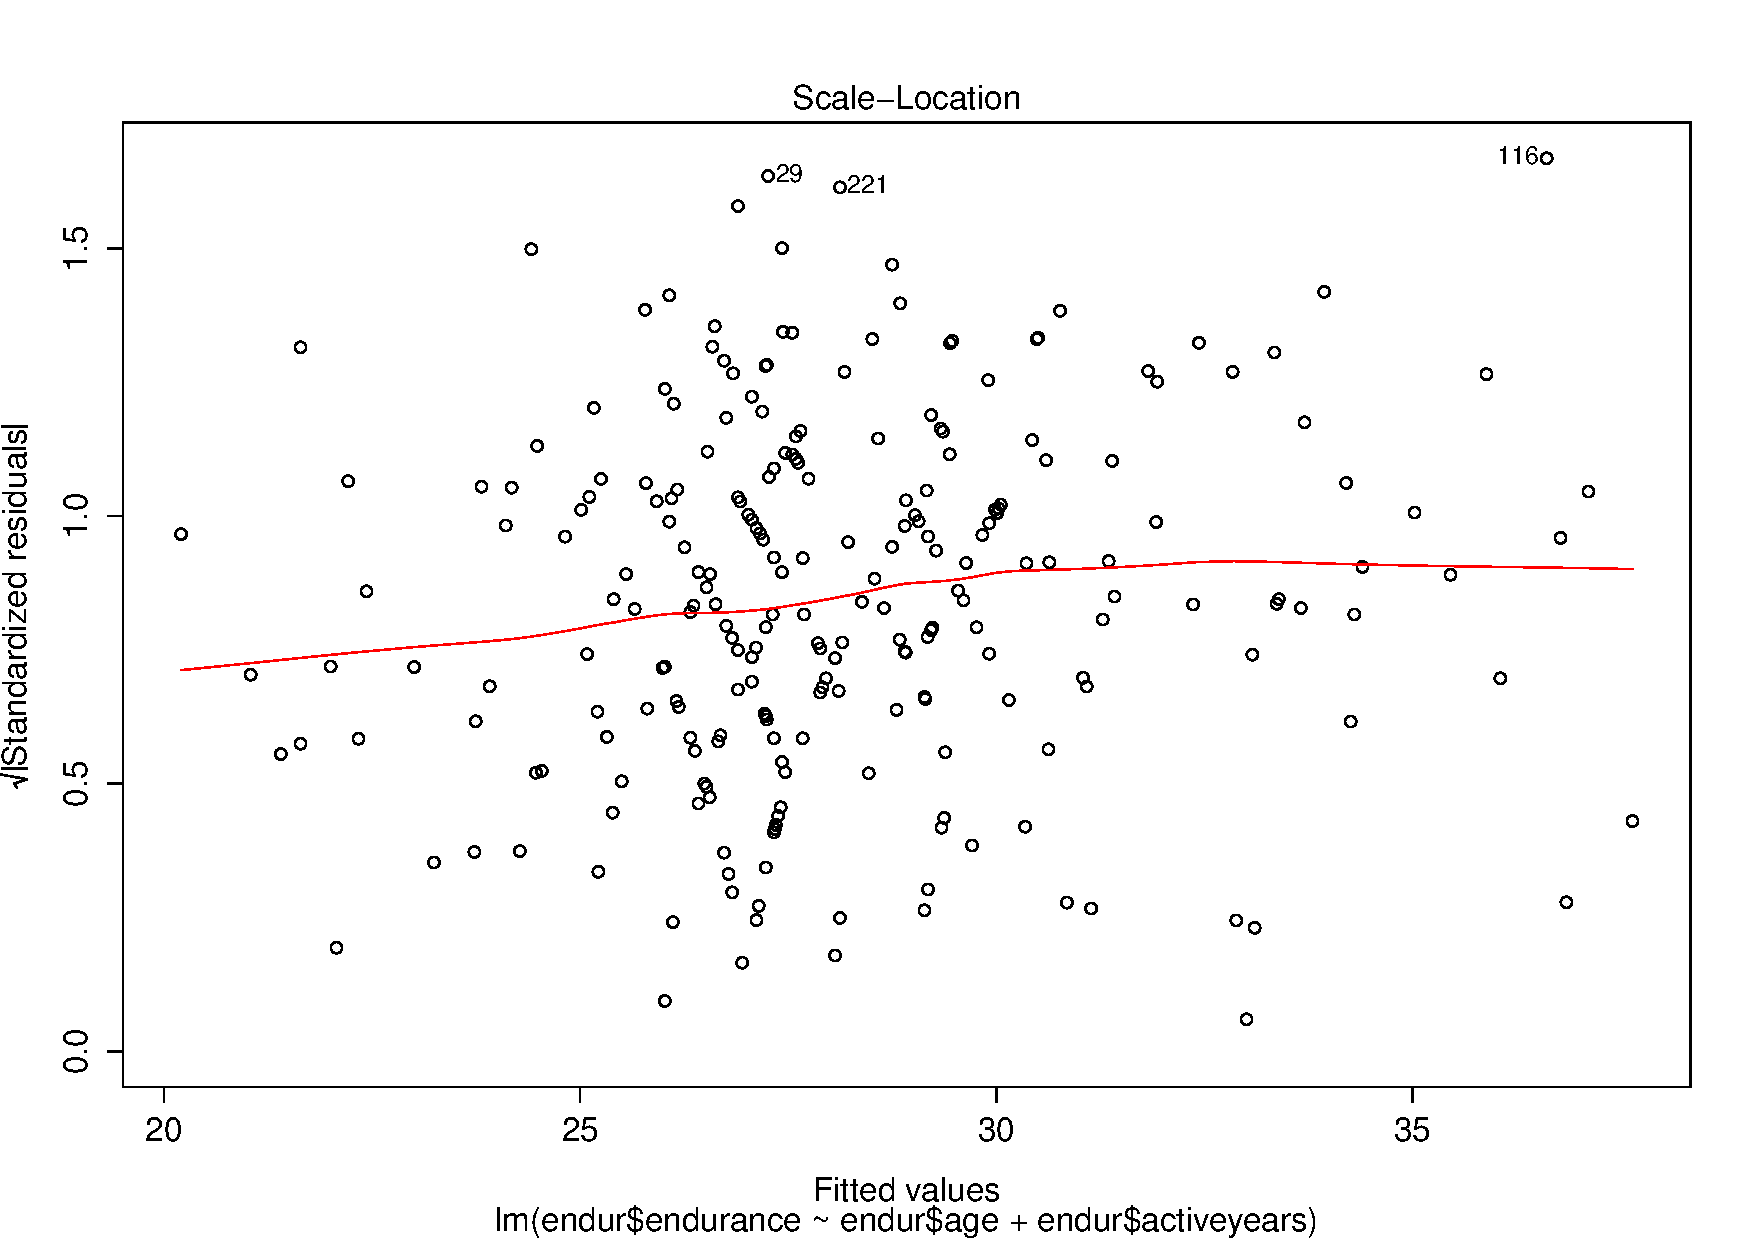
\includegraphics[width=0.8\textwidth]{Standardized-Residuals}\\
\end{figure}
\end{frame}












\section{Prévision}

\begin{frame}
\frametitle{Prévision}

Modèle de régression \vspace{2mm} \centerline{$ Y_i=
r(\truebeta, \alert{\bx}_i)+ \sigma \xi_i, \quad i=1,\dots,n.$}
Régression
\alert{linéaire}: $r(\truebeta, \alert{\bx}_i)=\truebeta^T
\bx_i$.
\begin{itemize}
\item \alert{Problème de prévision}:
Donner la prévison de la valeur de fonction de
régression $r(\truebeta,  \bx)=\truebeta^T \bx$\\
\item Soit $\estregress$ un estimateur de $\truebeta$. \alert{Prévision par
substitution:}
 \centerline{$\boxed{ \widehat Y(\bx) = r(\estregress, \alert{\bx}).}$}
\item \underline{Question statistique}: quelle est la qualité de la prévision?
\alert{Intervalle de confiance} pour $r(\estregress, \alert{\bx})$ ?
\end{itemize}
\end{frame}



\begin{frame}
\frametitle{Moyenne et variance de la prévision}
\begin{theorem}
\begin{itemize}
\item \alert<1>{$\PE_{\truetheta}[\hat{Y}_n(\bx)]= \bx^T \truebeta$}
\item \alert<2>{$\Var_{\truetheta}(\hat{Y}_n(\bx))= \sigma^2 \bx^T (\regressmat^T \regressmat)^{-1} \bx$}
\item \alert<3>{$\PE_{\truetheta}[ (Y(\bx) - \hat{Y}_n(\bx))^2]= \sigma^2 (1 + \bx' (\regressmat^T \regressmat)^{-1} \bx)$}
\end{itemize}
\end{theorem}
\only<1>{$\hat{Y}_n(\bx)= \bx^T \estregress$ et $\PE_{\truetheta}[\estregress]= \truebeta$}
\only<2>{
\begin{align*}
\hat{Y}_n(\bx)- \bx^T \truebeta&= \bx^T \regressmat^{\#} \bY - \bx^T \truebeta \\
&= \bx^T \regressmat^{\#} (\regressmat \truebeta + \sigma \bnoise) - \bx^T \truebeta = \sigma \bx^T \regressmat^{\#} \bnoise
\end{align*}
car $\regressmat^{\#} \regressmat= I$. Par conséquent, comme $\bX^{\#} \{ \bX^{\#} \}^T= (\bX^T \bX)^{-1}$,
$$
\Var_{\truetheta}(\hat{Y}_n(\bx))= \sigma^2 \bx^T \regressmat^{\#} \PE_{\truetheta}[\bnoise \bnoise^T] \{ \regressmat^{\#} \}^T \bx
$$}
\only<3>{
\begin{align*}
\PE_{\truetheta}[ (Y(\bx) - \hat{Y}_n(\bx))^2]
&= \PE_{\truetheta}[ (Y(\bx) - \PE_{\truetheta}[\hat{Y}_n(\bx)])^2] + \Var_{\truetheta}(\hat{Y}_n(\bx)) \\
&= \PE_{\truetheta}[ (Y(\bx) - \bx^T \truebeta)^2] +  \sigma^2 \bx^T (\regressmat^T \regressmat)^{-1} \bx
\end{align*}
}
\end{frame}


\begin{frame}
\frametitle{Prévision: modèle linéaire gaussienne}
\begin{prop}
Supposons que $\bnoise \sim {\mathcal N}(0,\sigma^2\mathrm{Id}_n)$.
\begin{enumerate}
\item $\widehat{Y}(\bx) \sim {\mathcal N}\big(\bx ^T\truebeta, \sigma^2 \bx^T \big(\regressmat^T\regressmat\big)^{-1} \bx \big)$
\item $\widehat{Y}(\bx)$ et $(\Id{n} - \projX) \bY$ sont
indépendants.
\end{enumerate}
\end{prop}
\end{frame}

\begin{frame}
\frametitle{Prévision: modèle linéaire gaussienne}
\begin{itemize}
\item D'après la Proposition,
$$
\eta:=\frac{\widehat{Y}(\bx) - \bx^T\truebeta}{\sqrt{\sigma^2 {\bx^T\big(\regressmat^T\regressmat\big)^{-1}\alert{\bx}}}}
\sim {\mathcal N}(0,1).
$$
\item On replace $\sigma^2$ inconnu par $\widehat \sigma_n^2 =
{\|(\Id{n}-\projX) \bY \|^2}/({n-k}).$
\item \alert{$t$-statistique:}
$$
t:= \frac{\widehat{Y}(\bx) -\alert{\bx}^T\truebeta}{\sqrt{\widehat
\sigma_n^2 \alert{\bx}^T\big(\regressmat^T\regressmat\big)^{-1}{
\bx}}}=\frac{\eta}{\sqrt{\chi/(n-k)}}\sim t_{n-k},
$$
\alert{loi de Student à $n-k$ degrés de liberté}, car $\eta\sim
{\mathcal N}(0,1)$, $\chi:=\|\boldsymbol{Y}-\regressmat
\estregress\|^2/\sigma^2\sim \chi^2(n-k)$ et $\eta \indep \chi$.
\end{itemize}
\end{frame}

\begin{frame}
\frametitle{Prévision: intervalle de confiance}
\begin{eqnarray*}
&&\PP \Big(-q_{1-\frac{\alpha}{2}}(t_{n-k}) \le \frac{\widehat Y
- \bx^T\truebeta} {\sqrt{\widehat \sigma_n^2  \bx^T\big(\regressmat^T\regressmat\big)^{-1} \bx }}\le
q_{1-\frac{\alpha}{2}}(t_{n-k})\Big) \\\hspace{4mm} &&= \PP(-
q_{1-\frac{\alpha}{2}}(t_{n-k}) \le t\le
q_{1-\frac{\alpha}{2}}(t_{n-k})) = 1-\alpha.
\end{eqnarray*}
$\Longrightarrow$ \alert{intervalle de confiance} de niveau
$1-\alpha$ pour $r(\truebeta,\bx)=\bx^T\truebeta$ est
\alert{$[r_L, r_U]$}, o\`u:
\begin{align*}
\alert{r_L}&=\widehat Y -
q_{1-\frac{\alpha}{2}}(t_{n-k})\sqrt{\widehat \sigma_n^2
\bx^T\big(\regressmat^T\regressmat\big)^{-1}\bx},\\
\alert{r_U}&= \widehat Y +
q_{1-\frac{\alpha}{2}}(t_{n-k})\sqrt{\widehat \sigma_n^2 \bx^T\big(\regressmat^T\regressmat\big)^{-1} \bx}.
\end{align*}
\end{frame}



\begin{frame}
\frametitle{Limites des moindres carrés et du cadre gaussien}
\begin{itemize}
\item Calcul \alert{explicite} (et efficace) de l'EMC  limité à
une fonction de régression \alert{linéaire}.
\item Modèle linéaire donne un cadre assez général:
\begin{itemize}
\item Modèle
polynomial, \item \alert{Modèles avec interactions...}
\end{itemize}
\item \alert{ Hypothèse de gaussianité} = cadre asymptotique implicite.
\item Besoin d'outils pour les modèles  à réponse \alert{$Y$ discrète}.
\end{itemize}
\end{frame}

%\section{Régression linéaire non-gaussienne}

\begin{frame}
\frametitle{Régression linéaire non-gaussienne} Modèle de
régression linéaire \vspace{3mm} \centerline{$ Y_i= \truetheta^T
\alert{x}_i+\xi_i, \quad i=1,\dots,n.$}

\vspace{-2mm}

\begin{itemize}
\item \underline{Hyp. 1'} : \alert{$\xi_i$ i.i.d., $\E[\xi_i]
=0$, $\E[\xi_i^2] = \sigma^2>0$.}
\item \underline{Hyp. 2'} : $\regressmat^T \regressmat>0$, \alert{$\lim_n\max_{1\le i \le n}\alert{x}_i^T
\big(\regressmat^T \regressmat\big)^{-1}\alert{x}_i =0$.}
\end{itemize}
\begin{prop}[Normalité asymptotique de l'EMC]
$$
\sigma^{-1}\big(\regressmat^T
\regressmat\big)^{1/2}(\estregress-\truebeta)\stackrel{d}{\longrightarrow}
{\mathcal N}\big(0, \mathrm{Id}_k), \quad n\to\infty.
$$
\end{prop}
\begin{itemize}
\item A comparer avec le cadre gaussien:\vspace{2mm}
\centerline{$\sigma^{-1}\big(\regressmat^T
\regressmat\big)^{1/2}(\estregress-\truetheta)\sim {\mathcal N}\big(0,
\mathrm{Id}_k)$ \text{pour tout $n$.}}
\end{itemize}
\end{frame}

%\begin{frame}
%\frametitle{Vitesses de convergence}
%\end{frame}

%\subsection{Propriété de l'EMC: cadre général (non-gaussien) }
%
%\begin{frame}
%\begin{itemize}
%\item \underline{Hyp. 1} : $\regressmat^T \regressmat$ inversible
%\item  \underline{Hyp. 2} :
%\alert{$\E\big[\bnoise\big]=0$,
%$\E\big[\bnoise\bnoise^T\big] = \sigma^2
%\mathrm{Id}_n$}.
%\end{itemize}
%\begin{prop}
%%Sous les hypothèses précédentes
%\begin{itemize}
%\item $\E_\truetheta\big[\estMC\big]=\truetheta$ et
%$$\E_\truetheta\big[\big(\estMC-\truetheta\big)\big(\estMC-\truetheta\big)^T\big]=\sigma^2 \big(\regressmat^T\regressmat\big)^{-1}$$
%\item Si l'on pose
%$$\boxed{\widehat \sigma_n^2 = \frac{\|\boldsymbol{Y}-\regressmat \estMC\|^2}{n-\alert{k}} = \frac{1}{n-\alert{k}}\sum_{i = 1}^n\big(Y_i-(\estMC)^T\bx_i\big)^2}$$
%alors $\E_\truetheta\big[\widehat \sigma_n^2\big]=\sigma^2.$
%\end{itemize}
%\end{prop}
%\end{frame}








\end{document}
== 